\chapter{Indicadores Sociais}
\section{}
\par Para identificar os níveis de pobreza de uma população, é primordial a classificação de aspectos para um padrão de vida digno e satisfatório, como dieta balanceada, vestimentas adequadas, acesso a serviços de saúde e educação, ambiente sadio, etc.
\par No Brasil, a Constituição Federal do Brasil de 1988, garante no Art. 6º que todos têm direitos sociais, estabelecendo dimensões para o bem-estar da população, como a educação, a saúde, a alimentação, o trabalho, a moradia, o transporte, o lazer, a segurança, a previdência social, a proteção à maternidade e à infância e a assistência aos desamparados.
\par Neste sentido, cabe a pergunta: Como andam os indicadores sociais tocantinenses levando em conta os últimos anos em que se teve um baixo crescimento do produto e consequentemente uma deterioração do mercado de trabalho? É possível ver na Figura 3.1 a evolução da taxa de pobreza do estado entre 2012 e 2019, comparando com o desempenho da região Norte e com o Brasil.
\begin{figure}[h]
	\caption{Taxa de Pobreza}
	\subcap{Linha de US\$5,50 PPC}
	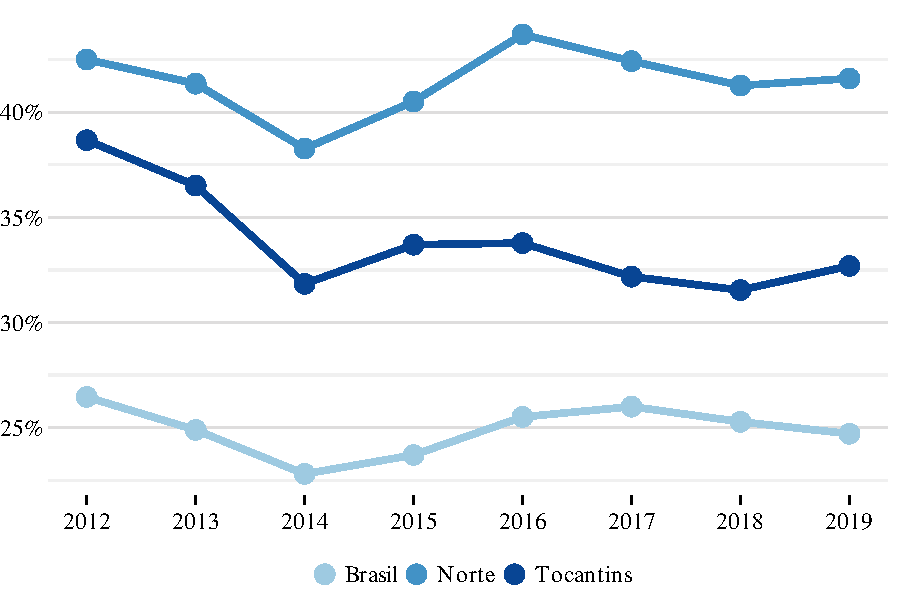
\includegraphics{fig/taxa_pobreza.pdf}
	\source{IBGE}
\end{figure}
\par Apesar do contexto apresentado na pergunta anterior, a taxa de pobreza do Tocantins apresentou uma queda de 38,67\% para 32,69\%, o que em números absolutos representou uma queda de 8,21\% de pessoas que saíram da linha da pobreza. Uma queda expressiva, ainda mais se comparada à média dos estados da região Norte, havendo inclusive um aumento da diferença com o nosso estado ao longo desses anos. Já se comparada à taxa brasileira, a taxa tocantinense ainda é maior, porém houve uma diminuição dessa diferença, uma vez que a taxa do nosso país não apresentou grandes oscilações nos anos analisados.
\par Cabe porém um destaque com relação aos dados relacionados ao ano de 2019. Neste ano, mesmo com uma queda da taxa brasileira de 25,28\% para 24,71\%, no estado do Tocantins houve um aumento da taxa saindo de 31,54\% para 32,69\%.

\begin{smbox}[label={labelbox},nameref={Taxas de Pobreza}]{Taxas de Pobreza}
	Uma das formas mais comuns de se mensurar pobreza é através de uma linha de pobreza absoluta, que define como pobres aqueles que vivem com uma renda inferior ao valor adotado pela linha. Neste sentido, o Banco Mundial sugere linhas que se adaptam melhor para as condições de vida de determinados países. Para um país de rendimento médio-alto, é sugerido uma linha de US\$5,50 PPC.  
\end{smbox}
\par Porém, olhando para uma faixa de renda menor ainda, a de extremamente pobres, os resultados não seguiram a mesma tendência, indicando um maior impacto do cenário apresentado para menores faixas de renda. Os resultados são apresentados na Figura 3.2.
\begin{figure}[h]
	\caption{Taxa de Extrema Pobreza}
	\subcap{Linha de US\$1,90 PPC}
	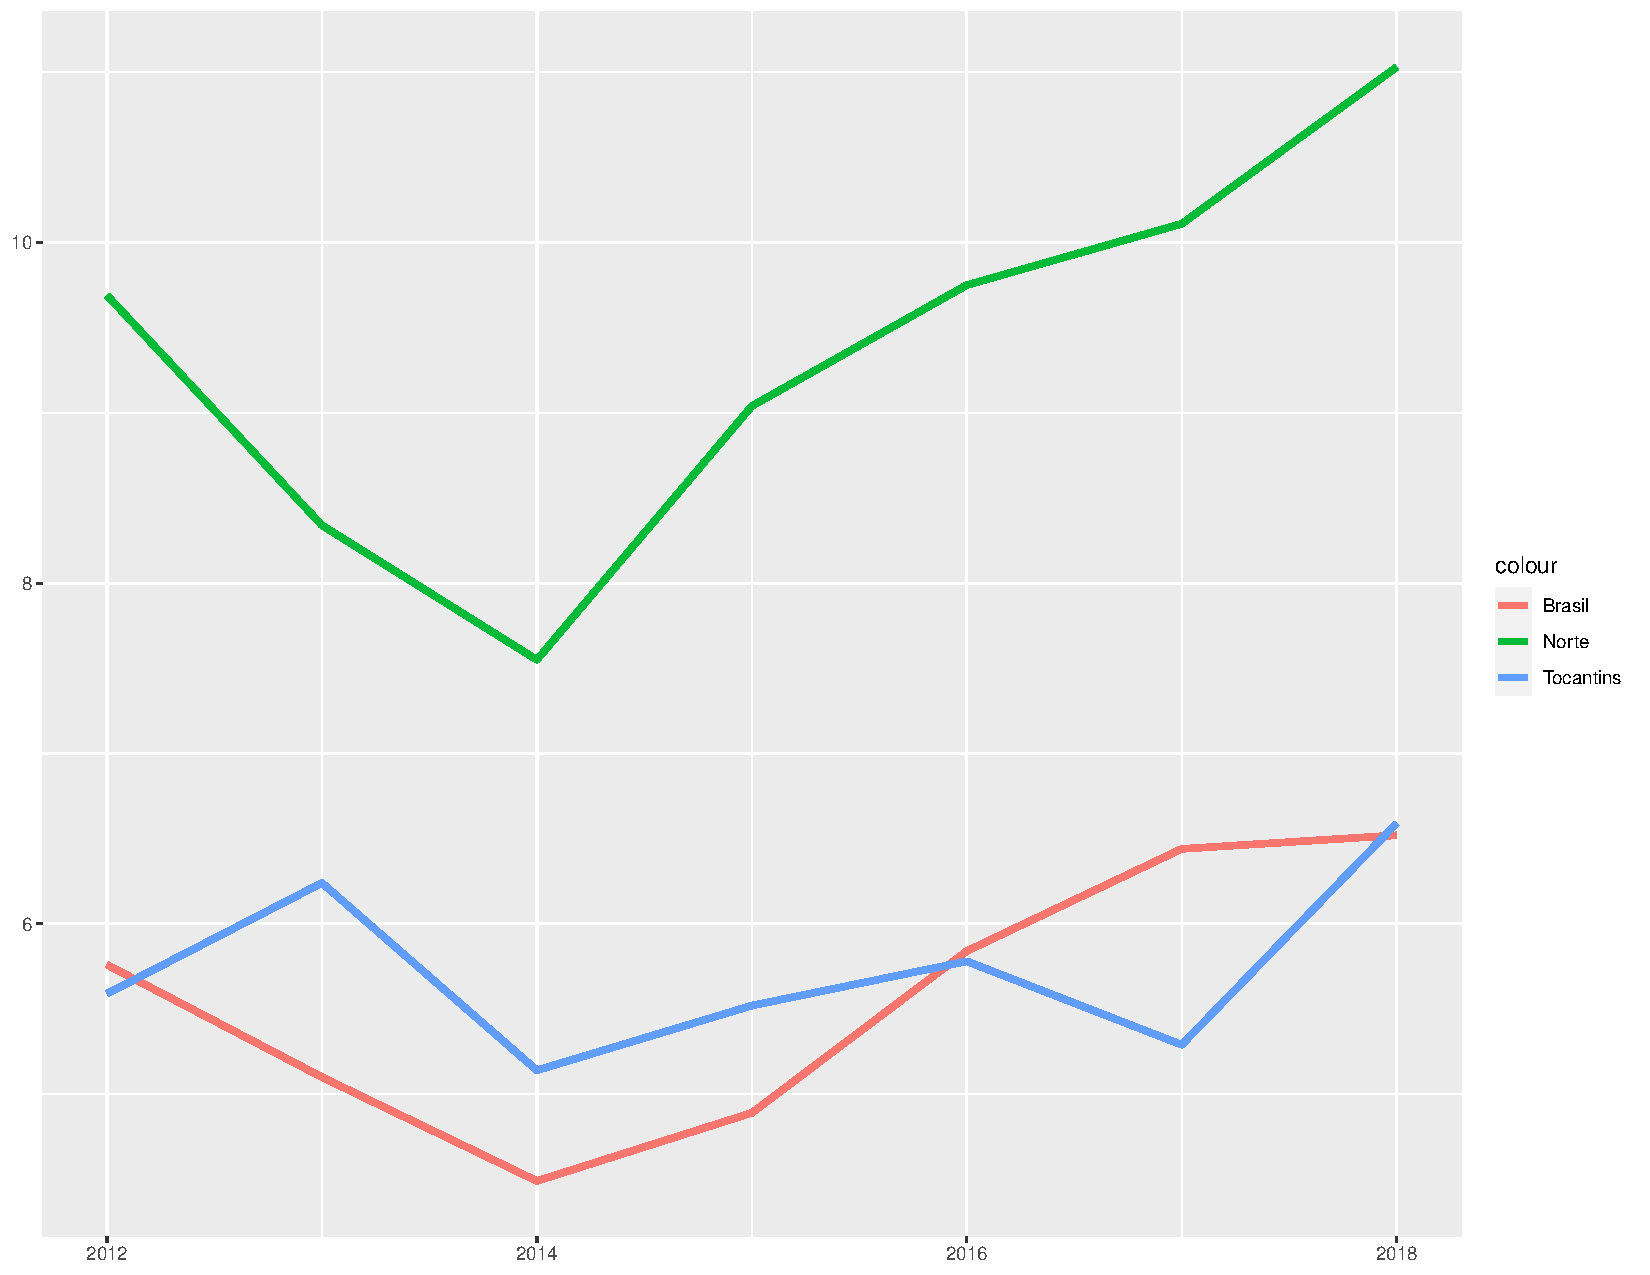
\includegraphics{fig/taxa_expobreza.pdf}
	\source{IBGE}
\end{figure}
\par A taxa de extrema pobreza apresentou alta entre 2012 e 2019 no estado, saindo de 5,59\% para 7,98\%. Em termos absolutos de pessoas vivendo nessa condição, tem-se a mínima em 2014 onde a partir daí ocorre uma alta de 64,35\%, um detalhe que em muitas vezes pode passar desapercebido olhando somente para a taxa que neste período saiu de 5,14\% para 7,98\%. O mesmo comportamento pode ser observado no indicador para o Brasil e  com mais intensidade ainda para região Norte.
\begin{figure}[h]
	\caption{Índice de Gini}
	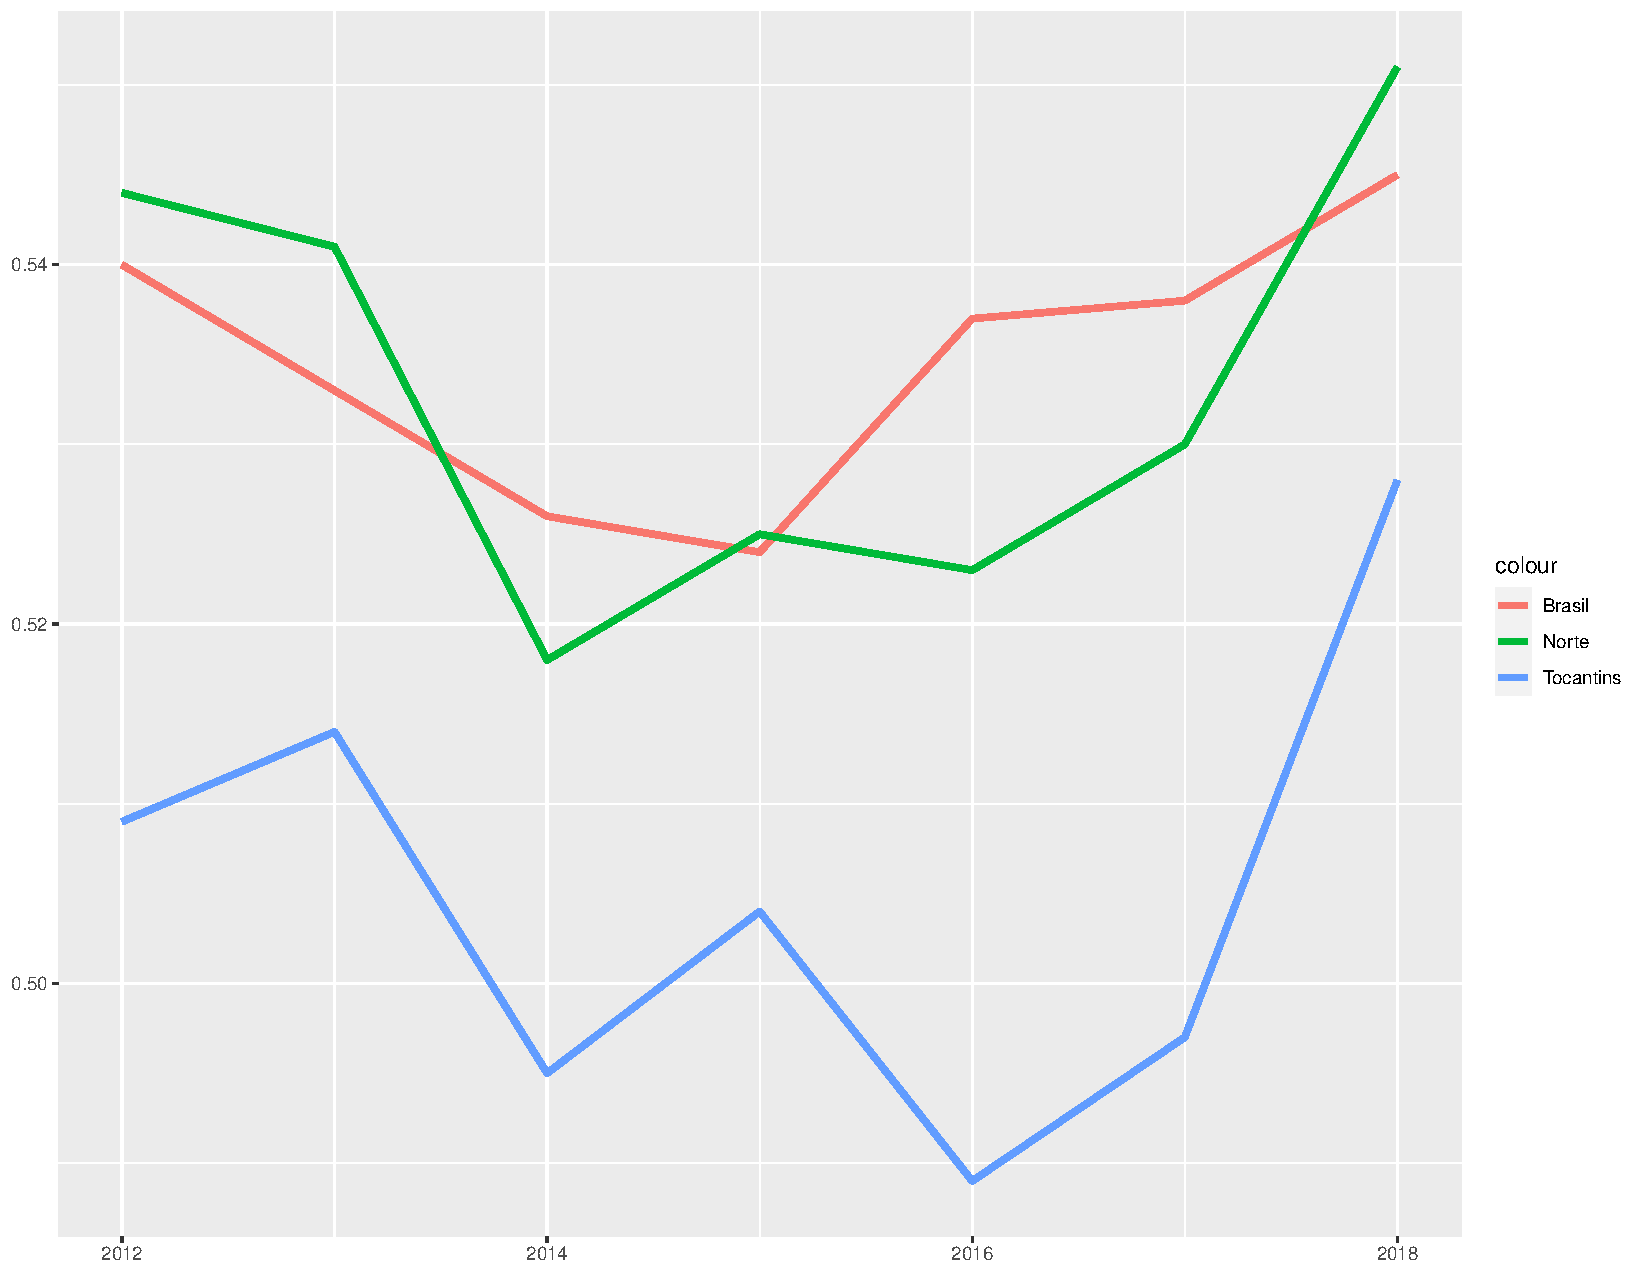
\includegraphics{fig/gini.pdf}
	\source{IBGE}
\end{figure}
\begin{smbox}[label={labelbox},nameref={Índice de Gini}]{Índice de Gini}
	É um índice que demonstra o grau de concentração de renda de um determinado grupo. Seus resultados variam entre 0 e 1. Quanto mais próximo de 0, mais igual é aquele grupo, e quanto mais próximo de 1, mas desigual é aquele grupo.
\end{smbox}
\par É possível perceber que houve uma leve alta do índice no nosso estado ao longo dos anos apresentados, saindo de 0,509 para 0,530, seguindo a tendência dos outros dados apresentados até então. Para o Brasil e para região Norte, idem. 
\par Os resultados apresentados nessa seção são produto, como já mencionado, do baixo crescimento econômico na década de 2010 e as suas consequências no mercado de trabalho, com aumento da taxa de desemprego, precarização dos trabalhos e aumento do trabalho informal. A crise fiscal enfrentada pela União e pelo estado do Tocantins de certa forma também contribuem para esse quadro, uma vez que gastos com programas sociais são muitas vezes cortados em contextos como este. Isso sem falar da baixa qualidade dos serviços públicos ofertados para a parte da população mais necessitada, o que de certa forma, perpetua o quadro apresentado aqui.
\par Superar as altas taxas de pobreza e desigualdade devem fazer parte de uma agenda para o estado do Tocantins possa ter uma economia mais forte, que cresça de forma mais sustentável e regular e para que o nosso povo viva cada vez melhor.  